\section{Synchronous Counters}
\label{sec:synchronous-counters}

\textit{Synchronous counters} are different from ripple counters in that clock pulses are applied to the inputs of all flip-flops. A common clock triggers all flip-flops simultaneously, rather than one at a time in succession as in a ripple counter.

\subsection{Binary Counter}
\label{subsec:binary-counter}

In a synchronous binary counter, the flip-flop in the least significant position is complemented with every pulse. A \textit{flip-flop in any other position is complemented when all the bits in the lower significant positions are equal to 1}. 

\noindent For example, if the present state of a four-bit counter is $A_3A_2A_1A_0 = 0011$, the next count is 0100. $A_0$ is always complemented. $A_1$ is complemented because the present state of $A_0 = 1$. $A_2$ is complemented because the present state of $A_1A_0 = 11$. However, $A_3$ is not complemented, because the present state of $A_2A_1A_0 = 011$, which does not give an all-1's condition.

Synchronous binary counters have a regular pattern of hardware elements and can be constructed with complementing flip-flops and gates. The regular pattern can be seen from the four-bit counter depicted in Fig. 12.

\begin{figure}[H]
  \centering
  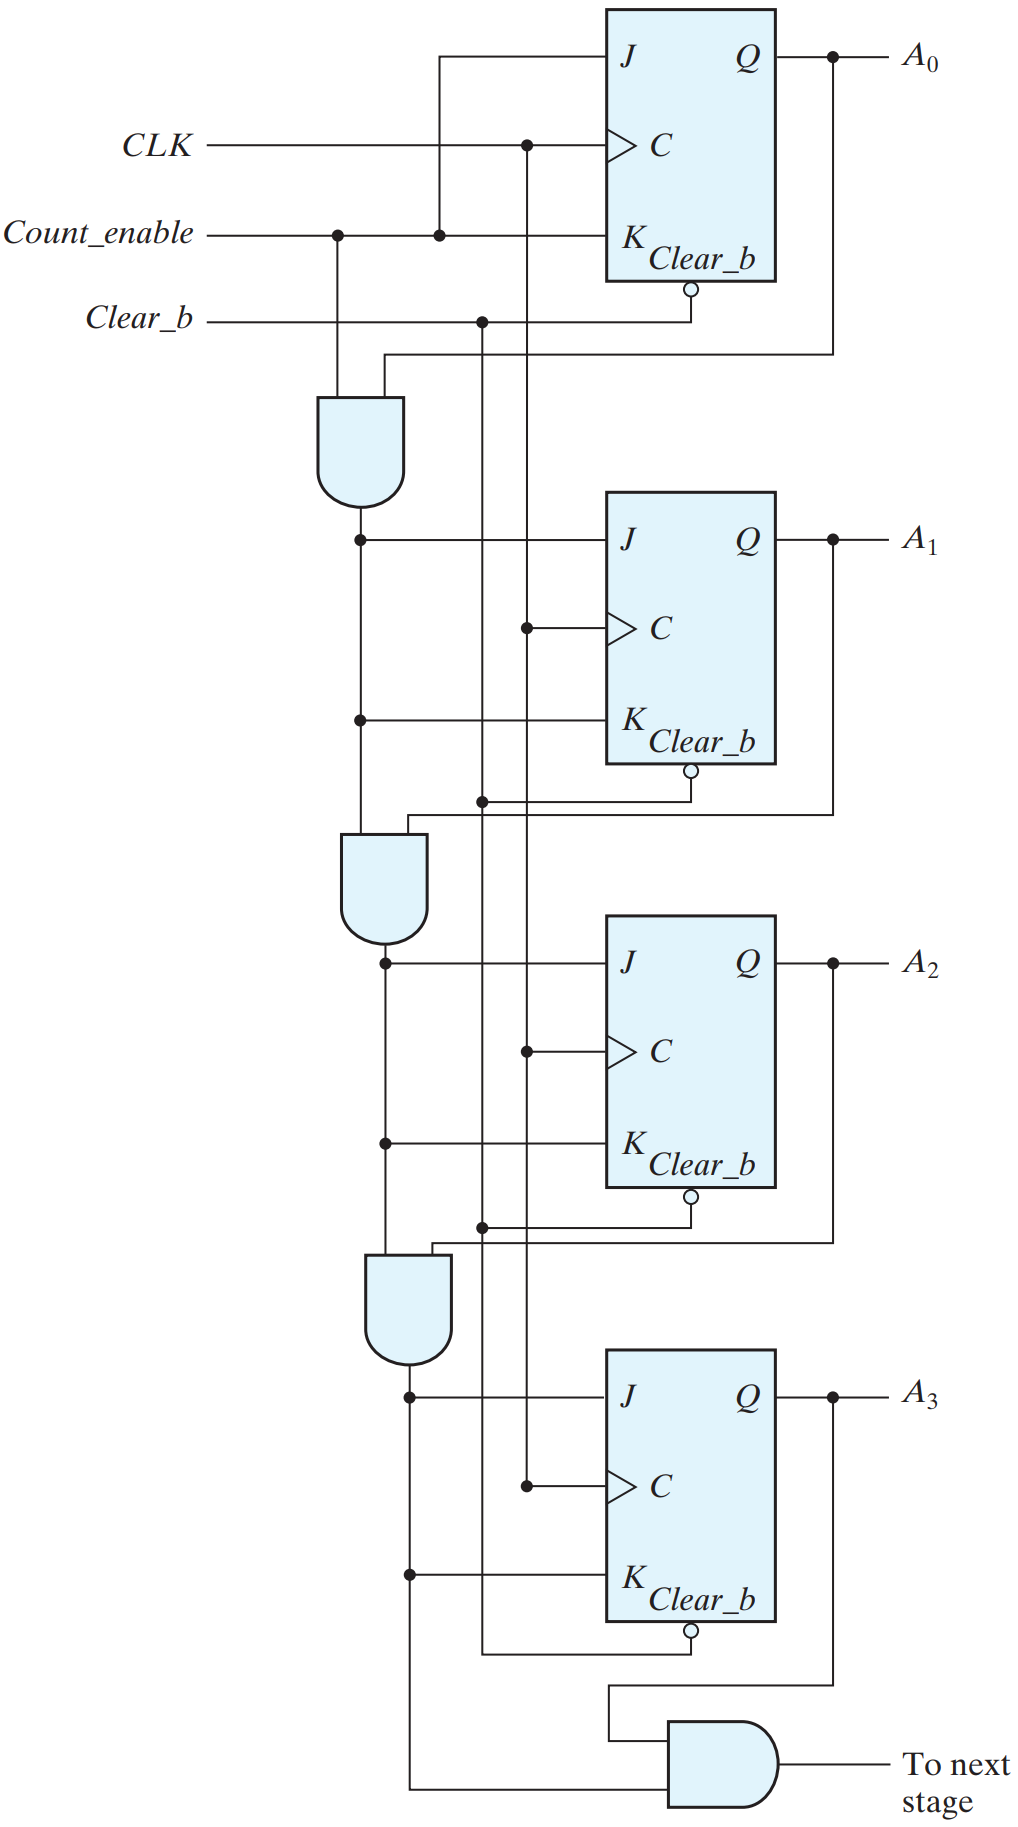
\includegraphics[width=.8\linewidth]{img/fig-6.12.png}
  \caption{Four-bit synchronous binary counter}
  \label{fig:6.12}
\end{figure}

The C (clock) inputs of all flip-flops are connected to a common clock.

\columnbreak

\subsection{Up–Down Binary Counter}
\label{subsec:up-down-binary-counter}

A synchronous countdown binary counter goes through the binary states in reverse order, from 1111 down to 0000 and back to 1111 to repeat the count.

The bit in the least significant position is complemented with each pulse. \textit{A bit in any other position is complemented if all lower significant bits are equal to 0}.

For example, the next state after the present state of 0100 is 0011. The least significant bit is always complemented. The second significant bit 
is complemented because the first bit is 0. The third significant bit is complemented because the first two bits are equal to 0. But the fourth bit does not change, because not all lower significant bits are equal to 0.

A countdown binary counter can be constructed as shown in Fig. 12, except that the inputs to the AND gates must come from the complemented outputs, instead of the normal outputs, of the previous flip-flops. The two operations can be combined in one circuit to form a counter capable of counting either up or down. The circuit of an up–down binary counter using T flip-flops is shown in Fig. 13.

When the \textit{up} input is 1, the circuit counts up, since the $T$ inputs receive their signals from the values of the previous normal outputs of the flip-flops. When the \textit{down} input is 1 and the \textit{up} input is 0, the circuit counts down, since the complemented outputs of the previous flip-flops are applied to the $T$ inputs. When the \textit{up} and \textit{down} inputs are both 0, the circuit does not change state and remains in the same count. When the \textit{up} and \textit{down} inputs are both 1, the circuit counts up.

\subsection{BCD Counter}
\label{subsec:bcd-counter}

A BCD counter counts in binary-coded decimal from 0000 to 1001 and back to 0000. The state table of a BCD counter is listed in Table 6.5. The input conditions for the $T$ flip-flops are obtained from the present- and next-state conditions. Also shown in the table is an output $y$, which is equal to 1 when the present state is 1001. In this way, $y$ can enable the count of the next-higher significant decade while the same pulse switches 
the present decade from 1001 to 0000.

The flip-flop input equations can be simplified by means of maps. The unused states for minterms 10 to 15 are taken as don't-care terms. The simplified functions are
\begin{align*}
  T_{Q_1} &= 1\\
  T_{Q_2} &= Q_8'Q_1\\
  T_{Q_4} &= Q_2Q_1\\
  T_{Q_8} &= Q_8Q_1 + Q_4Q_2Q_1\\
  y &= Q_8Q_1
\end{align*}
The circuit can easily be drawn with four $T$ flip-flops, five AND gates, and one OR gate.

\end{multicols}

\begin{figure}[H]
  \centering
  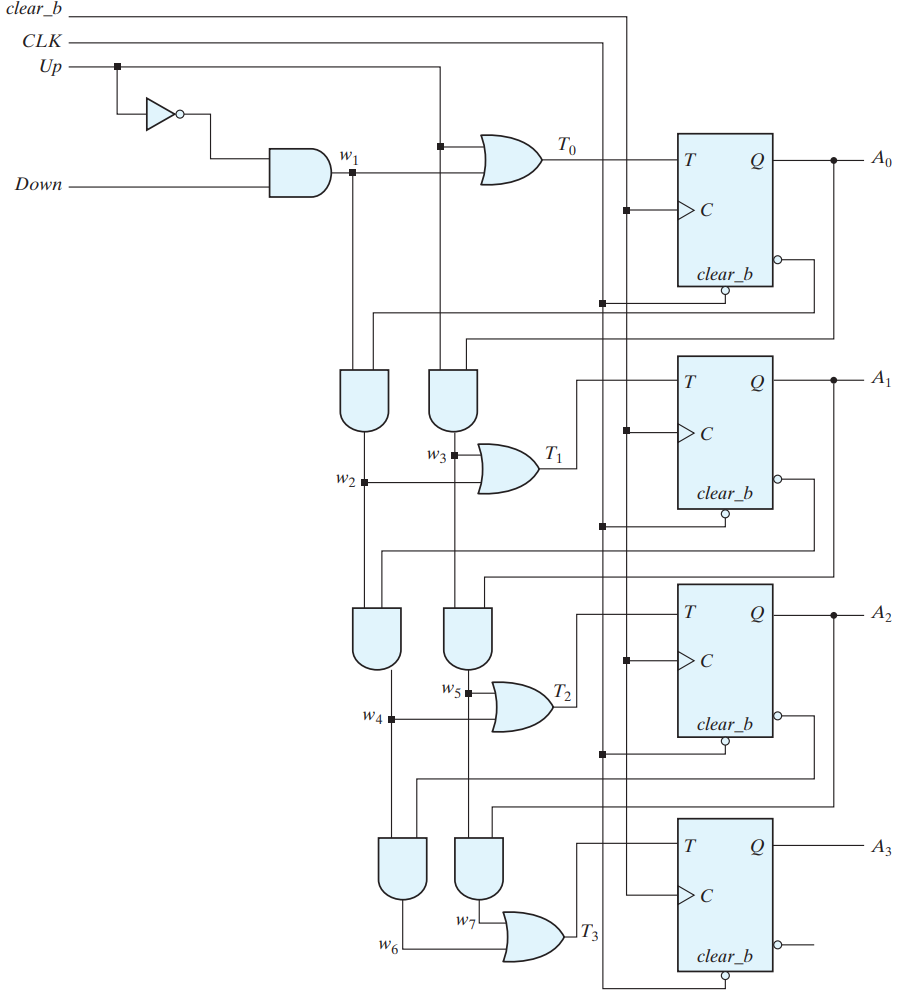
\includegraphics[width=.85\linewidth]{img/fig-6.13.png}
  \caption{Four-bit up–down binary counter}
  \label{fig:6.13}
\end{figure}

\noindent\rule{\textwidth}{1pt}

\begin{figure}[H]
  \centering
  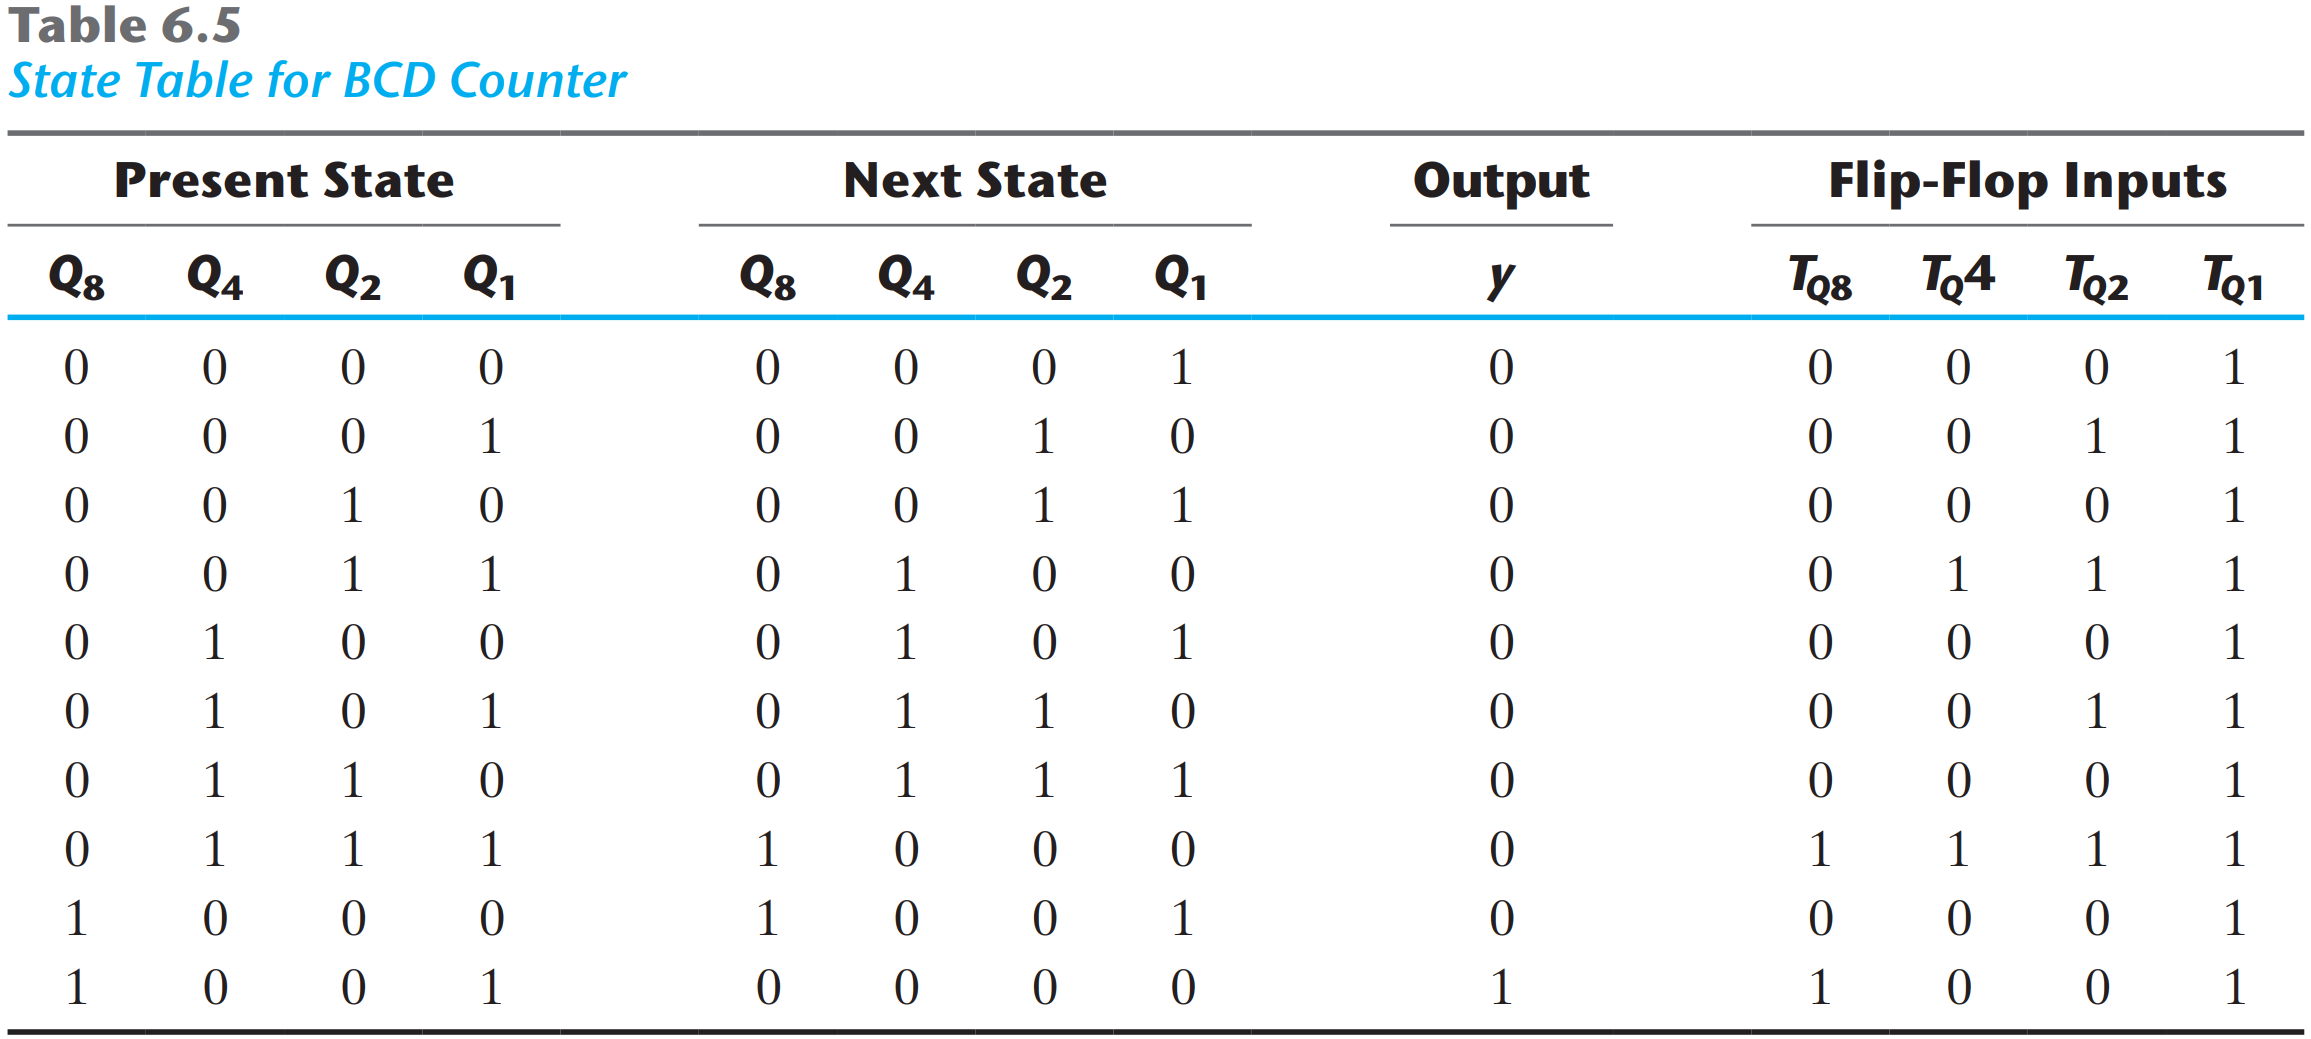
\includegraphics[width=.85\linewidth]{img/table-6.5.png}
  \label{table:6.5}
\end{figure}


\subsection{Binary Counter with Parallel Load}
\label{subsec:bin-counter-with-parallel-load}

Counters employed in digital systems quite often require a parallel-load capability for transferring an initial binary number into the counter prior to the count operation. Figure 14 shows the top-level block diagram symbol and the logic diagram of a four-bit register that has a parallel load capability and can operate as a binary counter.

\begin{figure}[H]
  \centering
  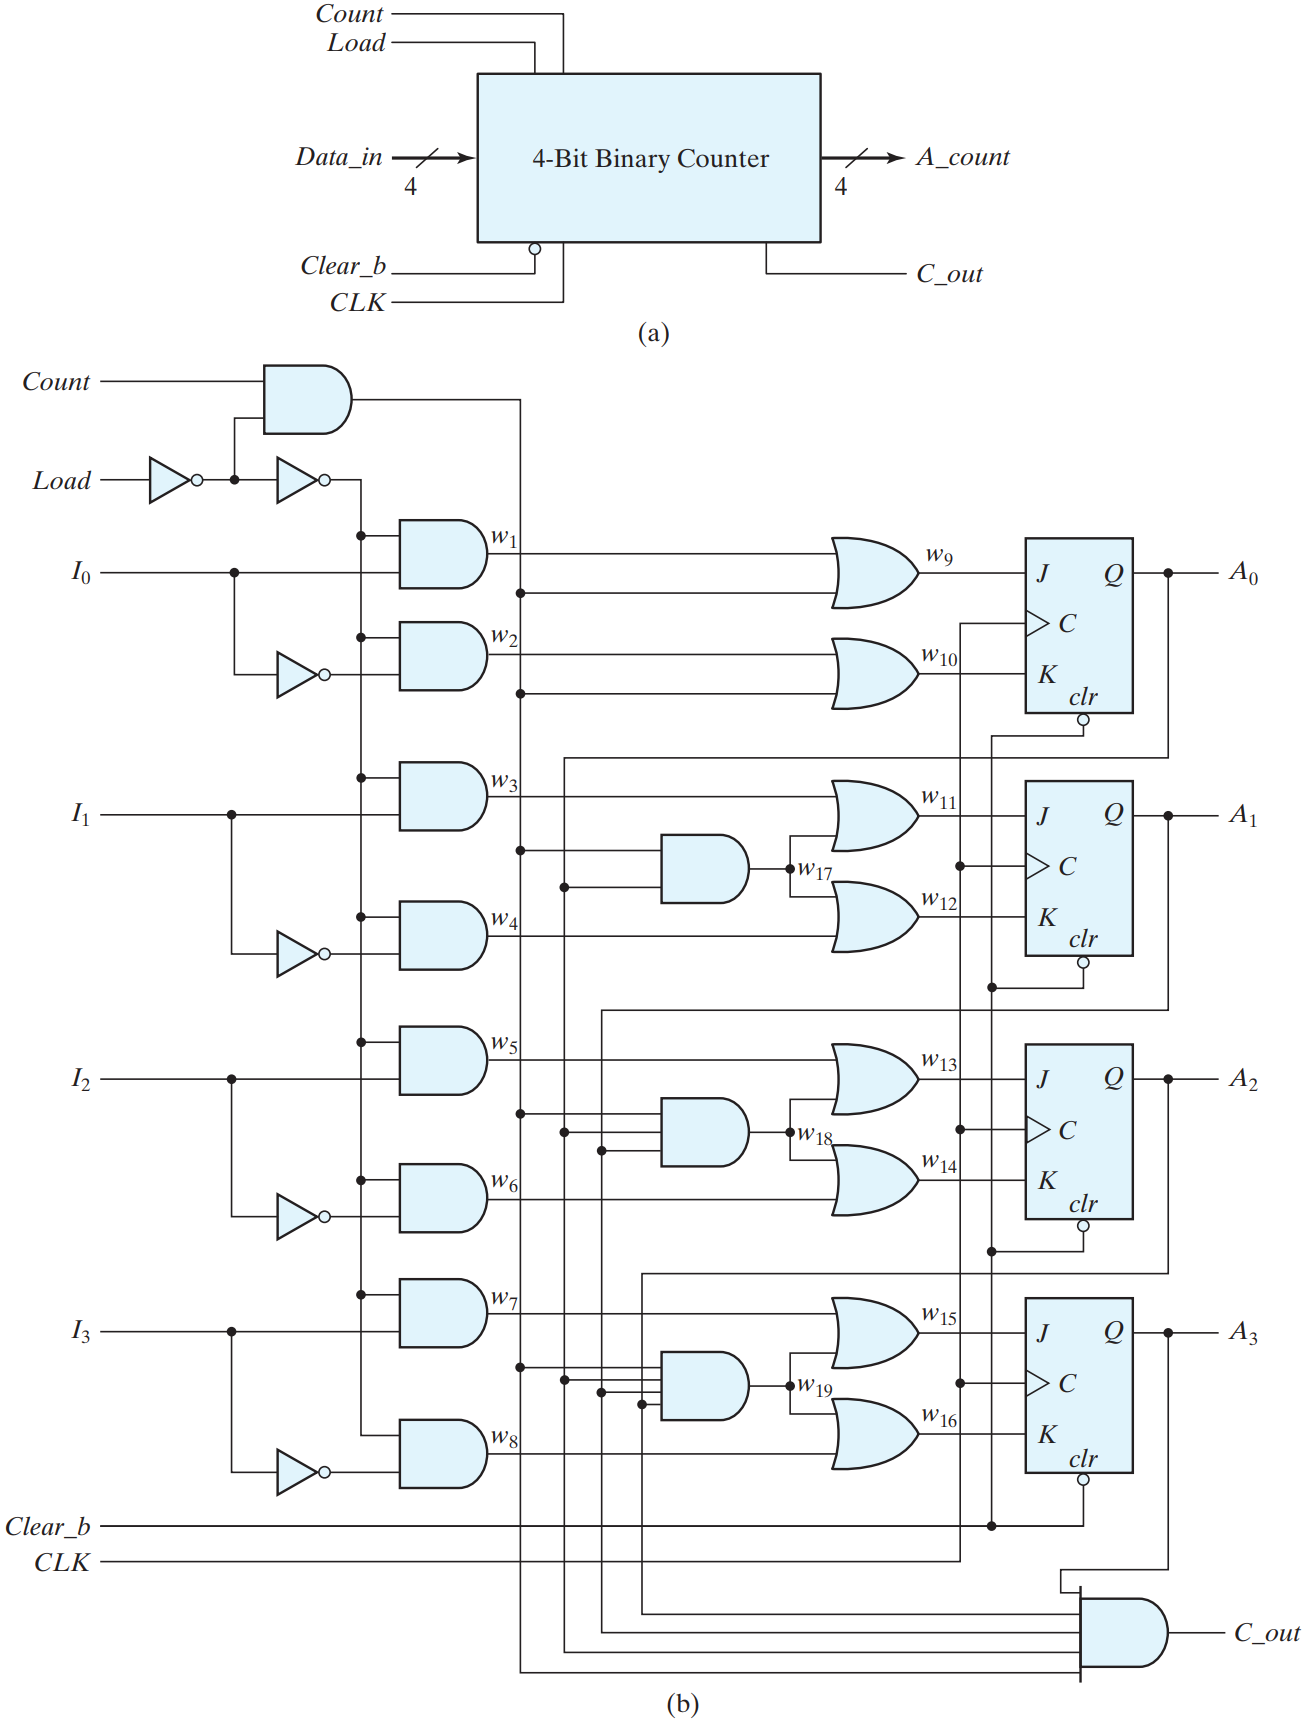
\includegraphics[width=.95\linewidth]{img/fig-6.14.png}
  \caption{Four-bit binary counter with parallel load}
  \label{fig:6.14}
\end{figure}

\begin{multicols}{2}
\setlength{\columnsep}{1.5cm}
\setlength{\columnseprule}{0.2pt}

\noindent The operation of the counter is summarized in Table 6.6.

\begin{figure}[H]
  \centering
  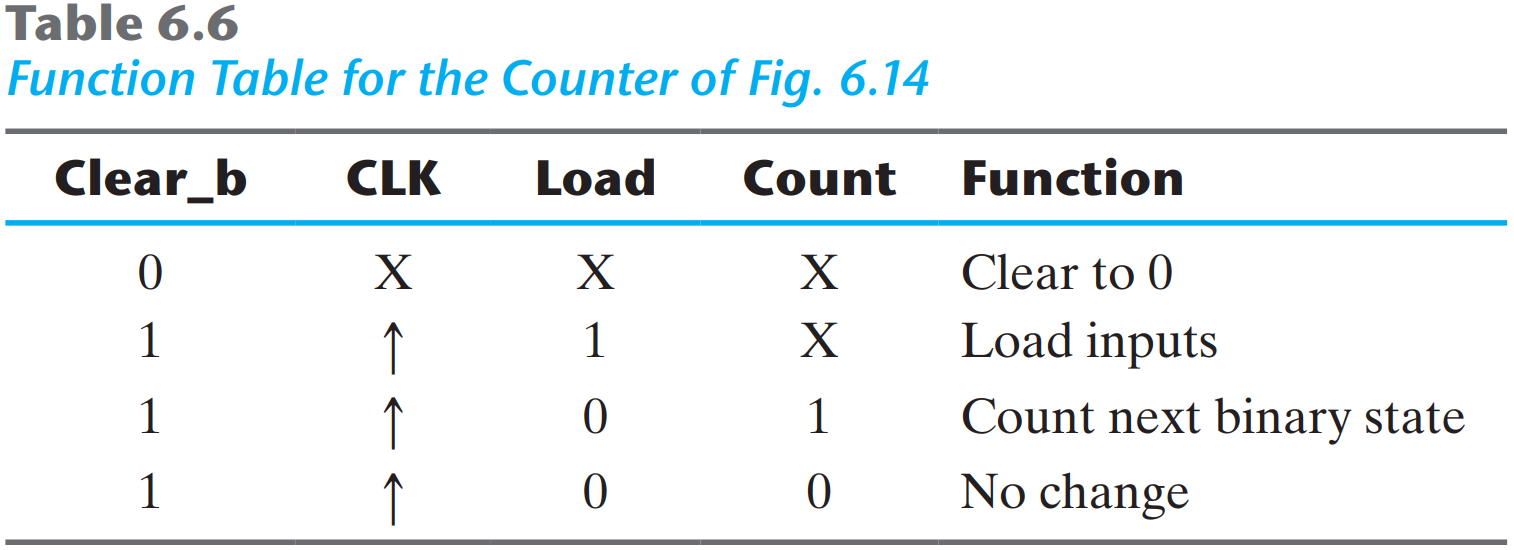
\includegraphics[width=\linewidth]{img/table-6.6.png}
  \label{table:6.6}
\end{figure}

A counter with a parallel load can be used to generate any desired count sequence. Figure 15 shows two ways in which a counter with a parallel load is used to generate the BCD count. In each case, the \textit{Count} control is set to 1 to enable the count through the \textit{CLK} input. Also, recall that the Load control inhibits the count and that the active-vlow clear action is independent of other control inputs.v

\end{multicols}

\begin{figure}[H]
  \centering
  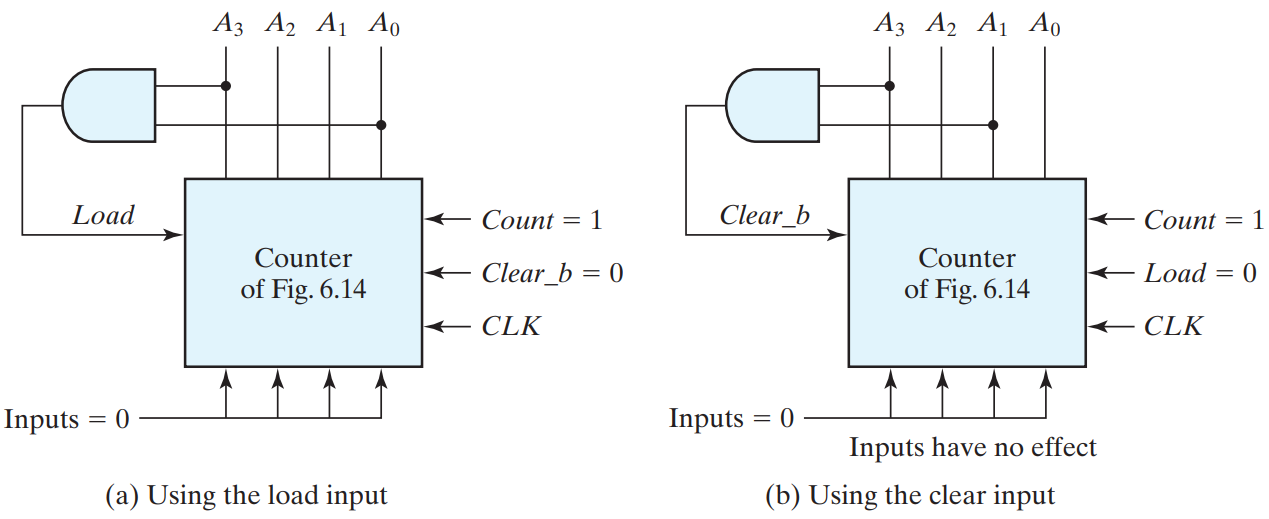
\includegraphics[width=.8\linewidth]{img/fig-6.15.png}
  \caption{Two ways to achieve a BCD counter using a counter with parallel load}
  \label{fig:6.15}
\end{figure}

\begin{multicols}{2}
\setlength{\columnsep}{1.5cm}
\setlength{\columnseprule}{0.2pt}

The AND gate in Fig. 15(a) detects the occurrence of state 1001($9_{10}$). At this count Load is asserted and 0s are loaded into the register at the next active edge of \textit{CLK}, effectively clearing the counter.

In the alternative counter shown in Fig. 15(b), the NAND gate detects the count of 1010($10_{10}$), but as soon as this count occurs, the register is cleared (asynchronously). The count 1010($10_{10}$) has no chance of staying on for any appreciable time, because the register goes immediately to 0.

\begin{practice}{Practice Exercise 6.3}
How do a ripple counter and a synchronous counter differ in their behavior? \\

\textbf{Answer:} 
All of the flip-flops in a synchronous counter are synchronized by receiving a common clock pulse; only the first stage of a ripple counter receives a clock pulse. The stages of a synchronous counter are updated simultaneous by a common clock; the stages of a ripple counter are updated one at a time. A synchronous counter operates faster than a ripple counter.
\end{practice}
